\documentclass[letterpaper, 10 pt, conference]{ieeeconf}  % Comment this line out if you need a4paper

%\documentclass[a4paper, 10pt, conference]{ieeeconf}      % Use this line for a4 paper

\IEEEoverridecommandlockouts                              % This command is only needed if 
                                                          % you want to use the \thanks command

\overrideIEEEmargins                                      % Needed to meet printer requirements.

%In case you encounter the following error:
%Error 1010 The PDF file may be corrupt (unable to open PDF file) OR
%Error 1000 An error occurred while parsing a contents stream. Unable to analyze the PDF file.
%This is a known problem with pdfLaTeX conversion filter. The file cannot be opened with acrobat reader
%Please use one of the alternatives below to circumvent this error by uncommenting one or the other
%\pdfobjcompresslevel=0
%\pdfminorversion=4

% See the \addtolength command later in the file to balance the column lengths
% on the last page of the document

% The following packages can be found on http:\\www.ctan.org1
%\usepackage{graphics} % for pdf, bitmapped graphics files
%\usepackage{epsfig} % for postscript graphics files
%\usepackage{mathptmx} % assumes new font selection scheme installed
%\usepackage{times} % assumes new font selection scheme installed
%\usepackage{amsmath} % assumes amsmath package installed
%\usepackage{amssymb}  % assumes amsmath package installed

\title{\LARGE \bf
Knowledge Graph Embedding in Multi-Agent Systems: A Distributed Control Perspective
}


\author{Sang-Won Kang${}^{1}$ and Hyo-Sung Ahn${}^{1*}$% <-this % stops a space
\thanks{*This work was not supported by any organization}% <-this % stops a space
\thanks{$^{1}$ School of Mechanical Engineering, Gwangju Institute of Science and Technology (GIST), Gwangju, Korea. 
        {\tt\small tony9707@gm.gist.ac.kr; hyosung@gist.ac.kr}}%
}

\usepackage{diagbox}
\usepackage{subcaption}
\usepackage{siunitx} % For units in tables
\usepackage[bottom]{footmisc}
\usepackage{physics}
\usepackage{amsmath,amsfonts,amssymb}
\newtheorem{theorem}{Theorem}[section]
\newtheorem{corollary}{Corollary}[theorem]
\newtheorem{lemma}[theorem]{Lemma}
\newtheorem{remark}{Remark}
\usepackage{graphicx}
\usepackage{tikz}
\usetikzlibrary{positioning, arrows}
\usetikzlibrary{arrows.meta}
\tikzset{mynode/.style={draw, very thick, circle, minimum size=1cm},
    myarrow/.style={very thick, -Triangle}}
% \usetikzlibrary{graphs, graphdrawing, arrows.meta}
% \usegdlibrary{force}



\begin{document}

\maketitle

\thispagestyle{empty}
\pagestyle{empty}

%%%%%%%%%%%%%%%%%%%%%%%%%%%%%%%%%%%%%%%%%%%%%%%%%%%%%%%%%%%%%%%%%%%%%%%%%%%%%%%%
\begin{abstract}
This paper proposes a novel framework that integrates Knowledge Graph Embedding (KGE) with distributed optimization and formation control in multi-agent systems. By focusing on TransE, we reformulate its optimization problem using the in-degree Laplacian matrix and distributed control theory, allowing agents to represent entities in the knowledge graph and interact only with neighboring entities. This framework offers a new perspective on embedding methods in decentralized environments and provides a foundation for future research in applying formation control to complex network structures. 
\end{abstract}


%%%%%%%%%%%%%%%%%%%%%%%%%%%%%%%%%%%%%%%%%%%%%%%%%%%%%%%%%%%%%%%%%%%%%%%%%%%%%%%%
\section{Introduction}
Knowledge Graph Embedding (KGE) has emerged as a powerful method for representing entities and relations in a continuous vector space. By embedding knowledge graphs, various downstream tasks such as link prediction, entity classification, and relation extraction are greatly enhanced \cite{wang_knowledge_2017}. Among the KGE techniques, TransE \cite{bordes_translating_2013} is one of the most popular and simplest methods, where relations between entities are modeled as translations in the embedding space. Despite its simplicity, TransE has performed remarkably in various knowledge graph tasks.

However, as the size and complexity of knowledge graphs grow, it becomes important to distribute the learning process among multiple agents, especially when dealing with decentralized or multi-agent systems. In such cases, traditional centralized optimization techniques may not be feasible. To address this, distributed optimization methods have gained significant attention in recent years. Distributed optimization allows each agent to focus on local objectives while collectively contributing to the global solution \cite{yang_survey_2019}. This makes it suitable for scenarios where agents have limited knowledge of the global network.

In this work, we propose a novel approach that connects TransE with distributed optimization and formation control. Our main result indicates how the TransE optimization problem can be formulated as a distributed optimization problem, where agents only interact with their neighbors. Furthermore, we demonstrate that the system's convergence can be analyzed using graph-theoretical tools, particularly the properties of the graph Laplacian. By drawing parallels with formation control in multi-agent systems, we establish a framework for understanding the dynamics of embedding in multi-agent settings.

The remainder of this paper is structured as follows: Section 2 provides the necessary preliminaries on graph theory and the TransE model. Section 3 presents our main results, illustrating the correspondence between KGE and formation control through both theoretical analysis and simulation. Finally, Section 4 concludes the paper with a discussion of the implications of our findings and potential directions for future research.

\section{Preliminaries}
This section introduces the essential concepts and mathematical tools that underpin our main results. We cover the basics of TransE, distributed optimization, and formation control, which will be used to derive our conclusions in the subsequent sections.

\subsection{Graph Theory}

Graph theory forms the foundation for modeling and analyzing the interactions and relationships in both knowledge graphs and multi-agent systems. In this work, we leverage graph theoretical concepts to unify the fields of Knowledge Graph Embedding (KGE) and formation control.

A \textbf{graph} \( G = (V, E) \) consists of a set of vertices \( V \) (or nodes) and a set of edges \( E \) that connect pairs of vertices. Each edge \( e \in E \) is an ordered pair \( (v_i, v_j) \), where \( v_i, v_j \in V \). In a \textbf{directed graph} (or digraph), edges have a direction, pointing from one vertex (the head) to another (the tail).

\subsubsection{Adjacency Matrix}

The \textbf{adjacency matrix} \( A \) of a graph \( G \) is a matrix where \( A_{ij} = 1 \) if there is a directed edge from vertex \( v_i \) to vertex \( v_j \), and \( A_{ij} = 0 \) otherwise. The adjacency matrix is crucial in representing the connectivity and structure of the graph, which directly impacts the behavior of vertices.

\subsubsection{Laplacian Matrix}

The \textbf{Laplacian matrix} \( L \) is derived from the adjacency matrix and plays a key role in understanding the graph's attributes \cite{mirzaev_laplacian_2013}. For a directed graph, the \textbf{in-degree Laplacian matrix} \( L \) is defined as:

\[
L = D - A
\]

\noindent where \( D \) is the diagonal matrix of in-degrees, with each diagonal element \( D(i, i) \) is equal to the in-degree of vertex \( v_i \), the number of edges directed towards \( v_i \).

\noindent The Laplacian matrix is fundamental in analyzing the dynamics of multi-agent systems, particularly in formation control, where it governs how agents influence each other based on the underlying graph structure.

In our work, $L$ is used to describe the linear couplings between entities in the knowledge graph. By analyzing the eigenvalues and eigenvectors $L$, we can infer whether the system converges to a stable solution or diverges in the embedding space.

\subsection{TransE}
TransE \cite{bordes_translating_2013} is a popular method for knowledge graph embedding that manages entities as vectors in a continuous space. Let $\mathcal{G} = (\mathcal{E}, \mathcal{R})$ be a knowledge graph where $\mathcal{E}$ is the set of entities and $\mathcal{R}$ is the set of relations. Given a triple $(h, r, t)$, where $h \in \mathcal{E}$ is the head entity, $t \in \mathcal{E}$ is the tail entity, and $r \in \mathcal{R}$ is the relation, TransE embeds $h$, $r$, and $t$ as vectors in $\mathbb{R}^d$ such that:
\[
\mathbf{h} + \mathbf{r} \approx \mathbf{t}
\]
Here, $\mathbf{h}$, $\mathbf{r}$, and $\mathbf{t}$ are the embedding vectors of $h$, $r$, and $t$, respectively. The objective function to minimize is typically formulated as:
\[
L(\mathcal{G}) = \sum_{(h,r,t) \in \mathcal{G}} \|\mathbf{h} + \mathbf{r} - \mathbf{t}\|_2^2
\]

This energy function drives the model to learn embeddings where the relational structure is preserved in the vector space. 

\subsection{Distributed Optimization}
In a distributed optimization framework, we consider a network of $N$ agents, where each agent $i$ has access to a local objective function $f_i(x_i)$ and interacts only with its neighboring agents in a communication graph. The global optimization problem is given by:
\[
\min \sum_{i=1}^{N} f_i(x_i)
\]
Each agent aims to minimize its own objective while exchanging information with neighboring agents to achieve a global consensus \cite{nedic_distributed_2009}. Distributed optimization is well-suited for large-scale systems where centralized optimization is impractical due to communication or computational constraints.

In this work, we interpret the TransE objective function as a distributed optimization problem where each agent corresponds to an entity in the knowledge graph and interacts with its neighbors via relation-specific and uni-directed interactions. The goal of each agent is to minimize the local objective derived from the TransE energy function while collectively achieving an embedding that satisfies the global structure of the knowledge graph.

\subsection{Formation Control}
Formation control is a widely studied problem in multi-agent systems where the goal is to drive a group of agents to achieve and maintain a desired formation \cite{oh_survey_2015}. The control law typically depends on the relative positions of the agents and can be written as:
\[
\dot{x}_i = k_p\sum_{j \in \mathcal{N}_i} (x_i - x_j - d_{ji})
\]
where $x_i$ is the position of agent $i$, $\mathcal{N}_i$ is the set of neighbors of agent $i$, and $d_{ij}$ is the desired relative displacement between agents $i$ and $j$. $k_p$ is a negative proportional gain of control law. The dynamics ensure agents converge to a formation that satisfies the specified relative displacements.

In the context of TransE, we draw an analogy between formation control and distributed optimization. The update rule for each agent in the optimization process can be viewed as a control law that governs the motion of entities in the embedding space. By leveraging tools from formation control theory, we can analyze the stability and convergence of the embedding process.

\section{Main Result}

\subsection{TransE and Distributed Optimization}
To adapt TransE for a distributed multi-agent system, we reformulated the optimization problem for each agent in the graph as follows:
\begin{subequations}
\begin{equation}\label{eq:min}
    \min \sum_{i=1}^{N} f_{i} (x_{i})
\end{equation}
\begin{equation}\label{eq:f_i}
    f_{i}(x_{i}) = \sum_{j \in \mathcal{H}_{i}} \frac{1}{2} \|x_{i} - x_{j} - r_{ji}\|_{2}^{2}
\end{equation}
\end{subequations}
In this context, \( x \in \mathbb{R}^{N \times d} \) denotes the embedding space of entities, where \( x_i \in \mathbb{R}^d \) is the embedding vector for the \(i\)-th agent out of \( N \) agents. The set \( \mathcal{H}_i \) includes the neighbors of agent \( i \), which serve as head entities. The vector \( r_{ji} \in \mathbb{R}^d \) signifies the predefined relation from entity \( j \) to entity \( i \). The objective is to minimize the energy function \( f_i \) for each agent. We assumed that the relation vectors are normalized to unit magnitude and are uni-directed. For simplicity, the embedding space \(x\) is assumed to be a column vector: \(x = [x_1, x_2, \ldots, x_n]^\top\) where \(x_i \in \mathbb{R}\) and \(r_ji \in \mathbb{R}\).

The optimization problem \eqref{eq:min} is addressed using a distributed optimization approach. Each agent aims to minimize its local objective function \eqref{eq:f_i}. The gradient of \( f_i \) with respect to \( x_i \) is given by:
\begin{equation}
    p_i = - \pdv{f_{i}}{x_{i}} = - \sum_{j \in \mathcal{H}_i} (x_{i} - x_{j} - r_{ji})
    \label{eq:p}
\end{equation}

The steepest descent direction \( p_i \) guides the optimization process towards a zero gradient. This is utilized in the Gradient Descent Method (GDM), where each \( x_i \) iteratively updates its position to reach a steady state:

\begin{equation}
    x_{i}^{t+1} = x_i^t + \alpha p_i(x_i^t)
    \label{eq:update}
\end{equation}

The step size \( \alpha \) regulates the update speed of agents. Although each agent may have its own local minimum, determining the stabilization of the entire system is challenging. Therefore, we expand \( p_i \) into a vector form:

\begin{equation}
    p = - (Lx - r)
    \label{eq:p_vector}
\end{equation}

Here, \( L \) represents the linear couplings between elements of \( x \), and \( r \) is a column vector containing all \( r_i \) (\( r_i = \sum_{j \in H_i} r_{ji} \)). Based on \eqref{eq:p_vector}, the original problem \eqref{eq:min} can be reformulated as:

\begin{equation}
    \min \frac{1}{2} \|Lx - r\|_{2}^{2}
    \label{eq:new_min}
\end{equation}
\noindent The solution \( x^* \) of \eqref{eq:new_min} implies that \( Lx^* - r = 0 \). % when the objective function is convex. 

In summary, TransE for multi-agent graphs can be seen as an optimization problem that can be solved in a distributed manner. Furthermore, spectral properties of the graph Laplacian \( L \) allow us to analyze the overall system behavior.

\subsection{Formation Control with Displacement}

The matrix \( L \) has specific properties, particularly regarding its singularity, which affects the existence of \( x^* \). To verify the system’s convergence, we utilize a method from formation control theory. The update rule in GDM \eqref{eq:update} plays a crucial role. 

\begin{remark}
    The update rule \eqref{eq:update} can be interpreted as a discrete-time approximation of the continuous-time dynamics of the system. By analyzing the continuous-time dynamics, we can determine the stability and convergence of the system. The dynamics of the system can be described as:

    \begin{equation}\label{eq:dis_dynamic}
        \dot{x}_i = k_p \sum_{j \in \mathcal{H}_i} (x_{i} - x_{j} - r_{ji})
    \end{equation}
    \begin{equation}\label{eq:total_dynamic}
        \dot{x} = k_p(Lx - r)
    \end{equation}
    \noindent \eqref{eq:total_dynamic} is a vector form of \eqref{eq:dis_dynamic}.
\end{remark}

The dynamics in \eqref{eq:total_dynamic} is a single integrator control law for displacement-based formation control of digraphs with a Laplacian matrix. As shown by the dynamics, the current state directly influences the rate of change. Thus, the previous distributed optimization problem and the new formation control problem are equivalent. Entities follow the control law \eqref{eq:total_dynamic}, making it possible to use control theory methods to analyze features of a new embedding system in continuous time.

Given the dynamics \eqref{eq:total_dynamic}, we derived another equation about agent's velocity:

\begin{equation}
    \ddot{x} = k_p L \dot{x}
    \label{eq:2dot}
\end{equation}

\noindent This differential equation has a simple solution:

\[ 
    \dot{x}(t) = e^{k_p Lt} \dot{x}_0 
\]

\noindent Since \( L \) is usually asymmetric and may have complex eigenvalues, we decompose \( L \) into Jordan form:

\[ 
    L = T J T^{-1} 
\]

\noindent where \( J \) is the Jordan form of \( L \). \( T \) and \(T^{-1}\) are the matrices of right and left laplacian eigenvectors and generalized eigenvectors. Substituting this into the solution:


\begin{equation}
    \dot{x}(t) = T e^{k_p J t} T^{-1} \dot{x}_0 
    \label{eq:jordan_decom}
\end{equation}
\noindent The matrix \( J \) has \( m \) zero eigenvalues \( \lambda_n = 0 \) (\( n = 1,2,...,m \)), and the real parts of the other nonzero eigenvalues are positive \cite{mirzaev_laplacian_2013}. As a result, only the zero eigenvalues affect the system's stability and convergence \cite{mesbahi_graph_2010}. 

%Moreover, velocity of the agents will converge to a steady state if algebraic multiplicity and geometric multiplicity of zero laplacian eigenvalues are the same. 

\subsection{Graph Laplacian Eigenvalues and Stability}
\begin{remark}
    When all zero laplacian eigenvalues have a simple \(1 \times 1 \) Jordan block, the velocity of the system will converge to a steady state. 
\end{remark} 

If 2 or more zero eigenvalues compose a bigger jordan block than \(1 \times 1\), the system will diverge because of nonzero elements on upper triangular part of the block. After the matrix exponential, the system will have polynomial terms of \(t\) which make the system diverge. For example, the matrix exponential of a \(3 \times 3\) Jordan block of zero eigenvalues is:
\[
\begin{matrix}
    \exp{\begin{bmatrix}
        0 & 1 & 0 \\
        0 & 0 & 1 \\
        0 & 0 & 0
    \end{bmatrix} k_p t} & = & 
    \begin{bmatrix}
        1 & k_p t & \frac{1}{2} (k_p t)^2 \\
        0 & 1 & k_p t \\
        0 & 0 & 1
    \end{bmatrix}
\end{matrix}
\]

On the right side of the equation, the polynomial terms of \(t\) will not vanish as time passes. Hence, the system velocity will diverge.

Hence, we explored the shapes of the graphs that produces the zero laplacian eigenvalues analyzed them if they have simple jordan blocks or not. We figured out two features of digraphs: \textbf{Roots} and \textbf{SCCs} (Strongly Connected Components).

\subsubsection{Roots}
A root acts solely as head entities without any external factors. For example, in Fig. \ref{fig:DAG}, the first entity is a root node that influences the second and fourth nodes by enforcing the relation vectors \( r_{12} \) and \( r_{14} \). Since roots have no incoming edges, the graph laplacian will have zero rows corresponding to the roots:

\begin{lemma}\label{lemma:q}
Let the \( z \)-th row of graph laplacian (\( L_z^\top\)) be a zero row. Then the left zero eigenvector \( q \) is given by:
\begin{equation}\label{eq:q}
    q = \{0, \dots, 0, \rho_z = 1, 0, \dots, 0\}^\top
\end{equation}
\noindent where \( \rho_z \) is the \( z \)-th element of \( q \).
\end{lemma}

\begin{proof}
\( L_z^\top \) is a zero row so it is linearly dependent. Therefore, we can find \( q \) to solve the equation \( q^\top L = \mathbf{0}_n^\top \). The result is \( q = \{0, \dots, 0, \rho_z = 1, 0, \dots, 0\}^\top \).
\end{proof}

We applied Lemma \ref{lemma:q} to graph laplacian jordan decomposition. We assumed that the first node of digraph is a root node. Then, the first row of graph laplacian is a zero row and \(T^{-1}\)'s will be \(q = \{1, 0, \dots , 0\}^\top \). 


\begin{theorem}
    Roots in a digraph generate zero laplacian eigenvalues with simple \(1 \times 1\) jordan blocks.
\end{theorem}

\begin{proof}
    Let the first row of graph laplacian be a zero row. Then, the left zero eigenvector \( q \) is given by \( q = \{1, 0, \dots , 0\} \) from Lemma \ref{lemma:q}. The jordan form of the graph laplacian is \( L = T J T^{-1} \) where \( T \) is the matrix of right eigenvectors and \( T^{-1} \) is the matrix of left eigenvectors. Since the first row of \( L \) is a zero row, the first row of \( T^{-1} \) is \( q \). 
    \begin{equation}\label{eq:J_1}
        J_1^\top = (T^{-1})_1^\top L T = q^\top L T = \mathbf{0}_N^\top T = \mathbf{0}_N^\top
    \end{equation}
    \noindent where \( J_1 \) is the first jordan block of \( L \). From \eqref{eq:J_1}, the first jordan block of \( L \) is a simple \(1 \times 1\) jordan block. Although there are other roots in the graph, they also have simple \(1 \times 1\) jordan blocks alike the first root.
\end{proof}

In conclusion, all roots in a digraph generate zero laplacian eigenvalues that have simple \(1 \times 1\) jordan blocks.

\subsubsection{SCCs}

Some nodes in a digraph are strongly connected to each other as they are reachable from other nodes. These nodes are called "Strongly Connected Components" (SCC). SCCs form subgraphs, where the nodes are mutually dependent. Fig. \ref{fig:DCG} illustrates an example SCCs forming a triangular cycle, where each node is both a head and a tail entity. The graph laplacian of a cycle has a one-dimensional kernel, resulting in one zero eigenvalue. The rows of the subgraph laplacian are linearly dependent, as there are no zero rows in the subgraph laplacian of SCCs. 

\begin{remark}
    A strongly connected subgraph in a digraph generates one zero laplacian eigenvalue. Therefore, zero eigenvalues from SCCs have \(1 \times 1\) jordan blocks. However, if a subgraph of SCCs is enforced by roots or other subgraphs of SCCs, its laplacian rows lose linear dependence as it has no zero eigenvalues. We named it as "Rooted SCCs". 
\end{remark}

Finally, we can rewrite \eqref{eq:jordan_decom} into:
\begin{equation}
    \dot{x}(t) \rightarrow \left( \sum_{n=1}^m p_n e^{-\lambda_n t} q_n^\top \right) \dot{x}_0 = \left( \sum_{n=1}^m p_n q_n^\top \right) \dot{x}_0
    \label{eq:solution}
\end{equation}

The solution \eqref{eq:solution} approaches a constant over time, where \( p_n \) and \( q_n \) are the right and left eigenvectors corresponding to \( \lambda_n \)  \cite{mesbahi_graph_2010}. 

\subsection{Convergence Analysis}

Given these features, we organized several cases of graphs for knowledge graph embedding: \textbf{Acyclic Digraphs} and \textbf{Cyclic Digraphs}.

\begin{figure}[h] % 'h' specifies placement (here)
    \centering
    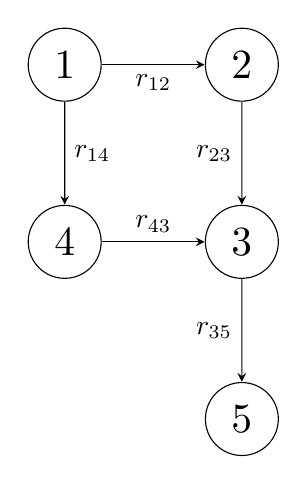
\begin{tikzpicture}[>=stealth, node distance=1.5cm]
    
    % Define nodes
    \node[circle, draw, fill=white!20, scale = 1.5] (1) {1};
    \node[circle, draw, fill=white!20, scale = 1.5, right of=1] (2) {2};
    \node[circle, draw, fill=white!20, scale = 1.5, below of=2] (3) {3};
    \node[circle, draw, fill=white!20, scale = 1.5, left of=3] (4) {4};
    \node[circle, draw, fill=white!20, scale = 1.5, below of=3] (5) {5};
    
    % Draw edges with arrows
    \draw[->] (1) -- (2) node[midway, below] {$r_{12}$};
    \draw[->] (2) -- (3) node[midway, left] {$r_{23}$};
    \draw[->] (1) -- (4) node[midway, right] {$r_{14}$};
    \draw[->] (3) -- (5) node[midway, left] {$r_{35}$};
    \draw[->] (4) -- (3) node[midway, above] {$r_{43}$};
    
    % Add labels to edges (optional)
    
    \end{tikzpicture} 
    \caption{A simple acyclic digraph with 5 nodes.}
    \label{fig:DAG}
    \end{figure}
\subsubsection{Acyclic Digraphs}

We defined an acyclic digraph as having some roots and rooted SCCs. These roots will strongly stabilize embedding result. 

\begin{theorem}
    Acyclic digraphs always converge to a steady state.
\end{theorem}

\begin{proof}
The root nodes \( x_n \) experience no external forces, so \( \dot{x}_n = 0 \). Furthermore, from Lemma \ref{lemma:q}, the left eigenvector \( q \) is \( \{1, 0, \dots, 0\} \). Substituting these into \eqref{eq:solution}, we found that the velocities of all agents goes to zero over time. 
\begin{equation}\label{eq:0_n}
    \dot{x} \rightarrow \sum_{n=1}^m p_n q_n^\top \dot{x}_0 = \sum_{n=1}^m (p_n \times 0) = \mathbf{0}_n
\end{equation}
This implies that the embedding of the acyclic digraph will converge to a steady state.
\end{proof}



\begin{figure}[h]
\centering
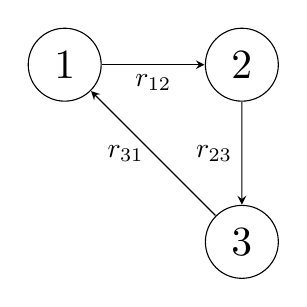
\begin{tikzpicture}[>=stealth, node distance=1.5cm]

% Define nodes
\node[circle, draw, fill=white!20, scale = 1.5] (1) {1};
\node[circle, draw, fill=white!20, scale = 1.5, right of=1] (2) {2};
\node[circle, draw, fill=white!20, scale = 1.5, below of=2] (3) {3};

% Draw edges with arrows
\draw[->] (1) -- (2) node[midway, below] {$r_{12}$};
\draw[->] (2) -- (3) node[midway, left] {$r_{23}$};
\draw[->] (3) -- (1) node[midway, left] {$r_{31}$};

% Add labels to edges (optional)


\end{tikzpicture}
\caption{A simple cycle of 3 SCCs.}
\label{fig:DCG}
\end{figure}



\subsubsection{Cyclic Digraphs}

We defined cyclic digraphs that contain no roots and all vertices in a cyclic digraph belong to a spanning tree so that only one zero laplacian eigenvalue appears. Its corresponding right eigenvector \( p \) is \( \mathbf{1}_n \) \cite{olfati-saber_consensus_2007}. \( k \) is arbitary and satisfies \( q^\top \dot{x}_0 = q^\top (-Lx(0) + r) = q^\top r = v \) (since \( q^\top L = 0 \)). In the case of cyclic digraphs, \eqref{eq:0_n} is replaced by \eqref{eq:v_n}.

\begin{equation}\label{eq:v_n}
    \dot{x} \rightarrow pq^\top \dot{x}_0 = \mathbf{1}_n \times v = \mathbf{v}_n
\end{equation}

\noindent Every agent in the cyclic graph acquires a uniform velocity \( v \). This behavior is known as \textbf{Velocity Alignment} \cite{dimarogonas_connection_2008}. If \( v = 0 \), the system will converge and the agents will reach \( x^* \). Otherwise, the agents diverge along linear paths:

\[
x(t) = \mathbf{v}_n t + X 
\]

\noindent while \( X \) is a constant vector from integration.


Even though the system remains unstable, the distances between heads and tails become steady because \( \dot{x}_i = \dot{x}_j \). Accordingly, the difference between agent $i$ and $j$ is organized as,
\[
x_i - x_j = (vt + X_i) - (vt +X_j) = X_i-X_j
\]
%We define this invariant relative formation $X$ as the embedding result in diverging cases.

To investigate more specifically, we concentrated on \eqref{eq:total_dynamic}. As the system works for a while, all velocities will become closed to \(v\). 

\begin{equation}\label{eq:findX}
\begin{split}
    \dot{x} &= k_p(Lx - r) \\
   \rightarrow  \mathbf{v}_n &= k_p(L(\mathbf{v}_nt + X) - r) \\
           &= k_p(LX - r)  \\ 
 \therefore X &= L^+ (r - \frac{\mathbf{v}_n}{k_p})
\end{split}
\end{equation}



Since \(q=\mathbf{1}_n\) is a right eigenvector of \(\lambda_1 = 0\), only \(X\) has left. We determined \( X \) from \eqref{eq:findX}, where \( + \) denotes the pseudo-inverse because the graph laplacian is singular. Followings are agent-based equations with respect to \(X\):

\begin{remark}
    The embedding results of cyclic digraphs are determined by \(X\), which is the relative formation of the agents. In addition, we orgainzed the relative formation of each agent \(X_i\) as following:
    \begin{equation}
        \begin{split}
        \dot{x}_i &= k_p(\sum_{j \in \mathcal{H}_i} (x_i - x_j) -r_i) \\
        \rightarrow v &= k_p(\sum_{j \in \mathcal{H}_i} (X_i - X_j) - r_i) \\
        X_i &= \frac{1}{|\mathcal{H}_i|}(\sum_{j \in \mathcal{H}_i} X_j +r_i-\frac{v}{k_p})
        \end{split}
    \end{equation}
\end{remark}



\subsection{Undirectional Embedding} 
We got inspiration from TransE to organize directional embedding formations of knowledge graphs. Tail entities are only enforced to move desired relative positions while heads receive no external forces. However, as we already mentioned, the embedding results will diverge for several cases because of unrooted SCCs. To stabilize them, we tried a new princeple: undirectional embedding.
\begin{equation}
    \dot{x}_i = k_p \sum_{j \in \mathcal{N}_i} (x_i - x_j - r_{ji})
\end{equation}

We expand the range of the node's neighbors to include its tails. That makes the system consider reverse relations. \( (t, -r, h) \). For reverse relations, we added a new condition: 

\[ r_{ij} = -r_{ji} \]

\noindent This condition indicates that the relation vector \( r_{ij} \) is the negative of \( r_{ji} \). The new condition ensures that the system is stable and converges to a steady state.

A connected undirected graphs always has a symmetry graph laplacian that involves only one zero eigenvalue and \( p = 1_n \) \cite{olfati-saber_consensus_2007}. According to \eqref{eq:2dot} and \eqref{eq:solution}, all agent's velocity also converge to \(q^\top r\) where \(q = \mathbf{1}_n / N \). 

\[
q^\top r = \frac{1}{N} \sum_{i = 1}^N r_i = 0
\]

\noindent Its result is finally zero. (\(\because r_{ji} = -r_{ij}\)). Consequently, undirected knowledge graphs have settled embedding results. 

\section{Simulation}
We conducted computer simulations of embedding formations for several knowledge graphs. These simulations focus on how agents move over time, providing complementary insights to our main analysis.

The embedding space is composed of \(x\) and \(y\) coordinates, with all entities starting from random initial positions. The agents update their positions using the Euler method with a step size of \(0.001\). The simulation ends when the agents reach a steady state, where the change in position is negligible. The results are visualized using \textbf{MATLAB}.

\begin{figure}[thb]
    \begin{center}
    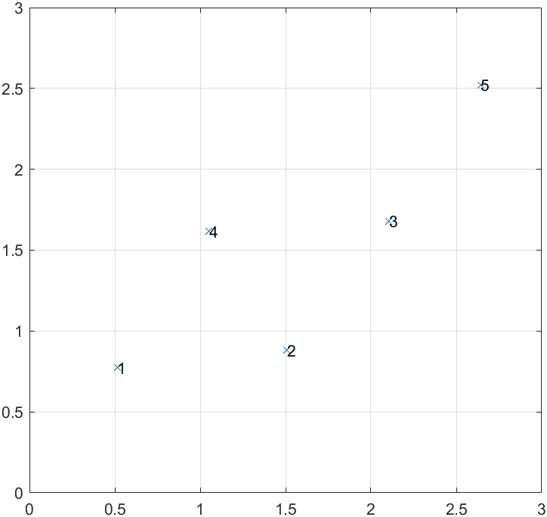
\includegraphics[width=7cm]{IMG/AG_simul3.png}
    \caption{A converging acyclic digraph composed of 5 entities.}
    \label{fig:DAGstate}
    \end{center}
    \vspace{-0mm}
\end{figure}




First, we performed the embedding of the graph shown in Fig. \ref{fig:DAG}. The five entities converged to their respective embedding points as illustrated in Fig. \ref{fig:DAGstate}. Entity \(E_1\) remained at its initial position since it is the root node. The other four entities adjusted their positions relative to this anchor point.
\begin{equation}\label{eq:result1}
\begin{split}
    E_2 &= E_1 + r_{12}\\
    E_3 &= E_1 + \frac{r_{12}+r_{23}+r_{14}+r_{43}}{2}\\
    E_4 &= E_1 + r_{14}\\
    E_5 &= E_1 + \frac{r_{12}+r_{23}+r_{14}+r_{43}}{2} + r_{35}
\end{split}
\end{equation}



\noindent The outcome \eqref{eq:result1} accomplishes \(Lx^* - r = 0\). 


Fig. \ref{fig:velo_align} shows the velocity alignment of a cyclic digraph with 3 entities. They initiated with distinct state but gradually made consensus so that the agents may keep moving in parallel. This behavior is a characteristic of cyclic digraphs and demonstrates how the embedding process can be analyzed using formation control principles.



\begin{figure}[thb]
    \begin{center}
    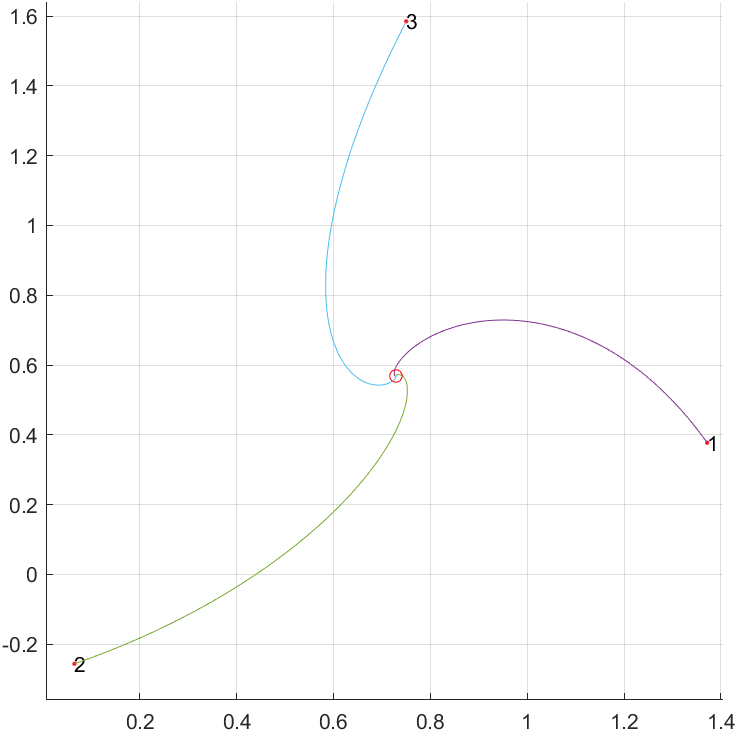
\includegraphics[width=7cm]{IMG/node3_velo_align_4.png}
    \caption{A cyclic digraph composed of 3 entities. Velocity alignment occurs.}
    \label{fig:velo_align}
    \end{center}
    \vspace{-0mm}
\end{figure}

\begin{figure*}[h] % 'h' specifies placement (here)
    \centering
    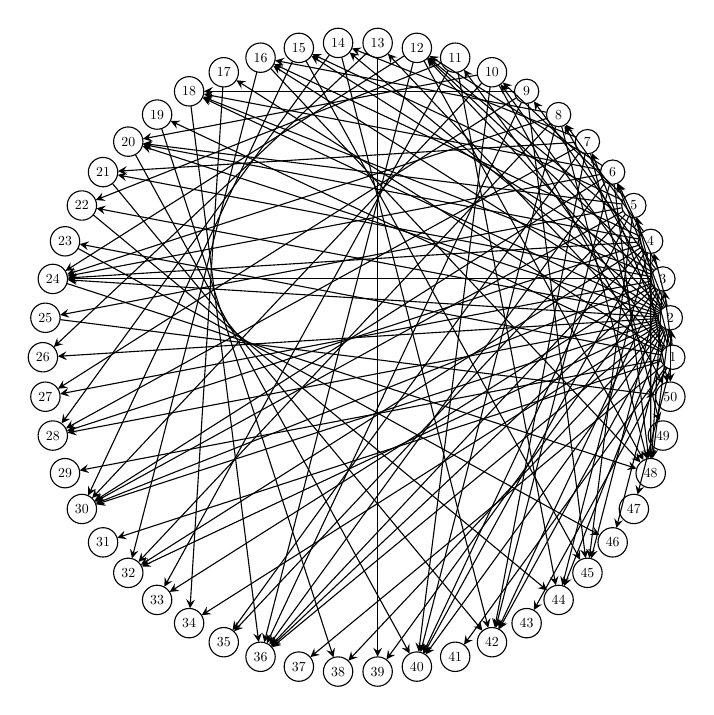
\begin{tikzpicture}[>=stealth, node distance=1.5cm]
    
    % Define nodes
    % \foreach \i in {1,...,50} {
    %     \node[circle, draw, fill=white!20, scale=1.5] (\i) at (0,0) {\i};
    % }
    \foreach \i in {1,...,50} {
        \node[circle, draw, fill=white!20, scale=0.5] (\i) at ({360/50 * (\i-1)}:4cm) {\i};
    }
    
    % Draw edges with arrows
    \foreach \i in {2, 3, 5, 7, 11, 13, 17, 19, 23, 29, 31, 37, 41, 43, 47} {
        \draw[->] (1) -- (\i);
    }

    \foreach \i in {2,...,50} {
        \foreach \j in {2,...,50} {
            \pgfmathtruncatemacro{\multiple}{\i*\j}
            \ifnum\multiple<51
                \draw[->] (\i) -- (\multiple);
            \fi
        }
    }
    % Add labels to edges (optional)
    
    \end{tikzpicture}
    \caption{Acyclic digraph of 50 nodes.}
    \label{fig:50nodes}
\end{figure*}





\begin{figure*}[h]
    \begin{center}
    \begin{subfigure}[b]{0.45\textwidth}
        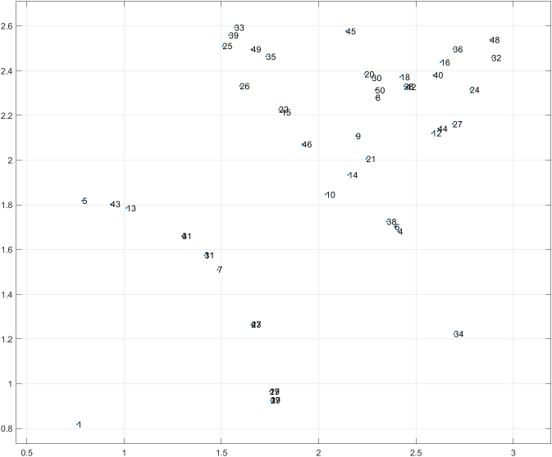
\includegraphics[width=\textwidth]{IMG/ag_50nodes.png}
        \caption{Embedding of an acyclic digraph with 50 nodes.}
        \label{fig:ag_50nodes}
    \end{subfigure}
    \hfill
    \begin{subfigure}[b]{0.45\textwidth}
        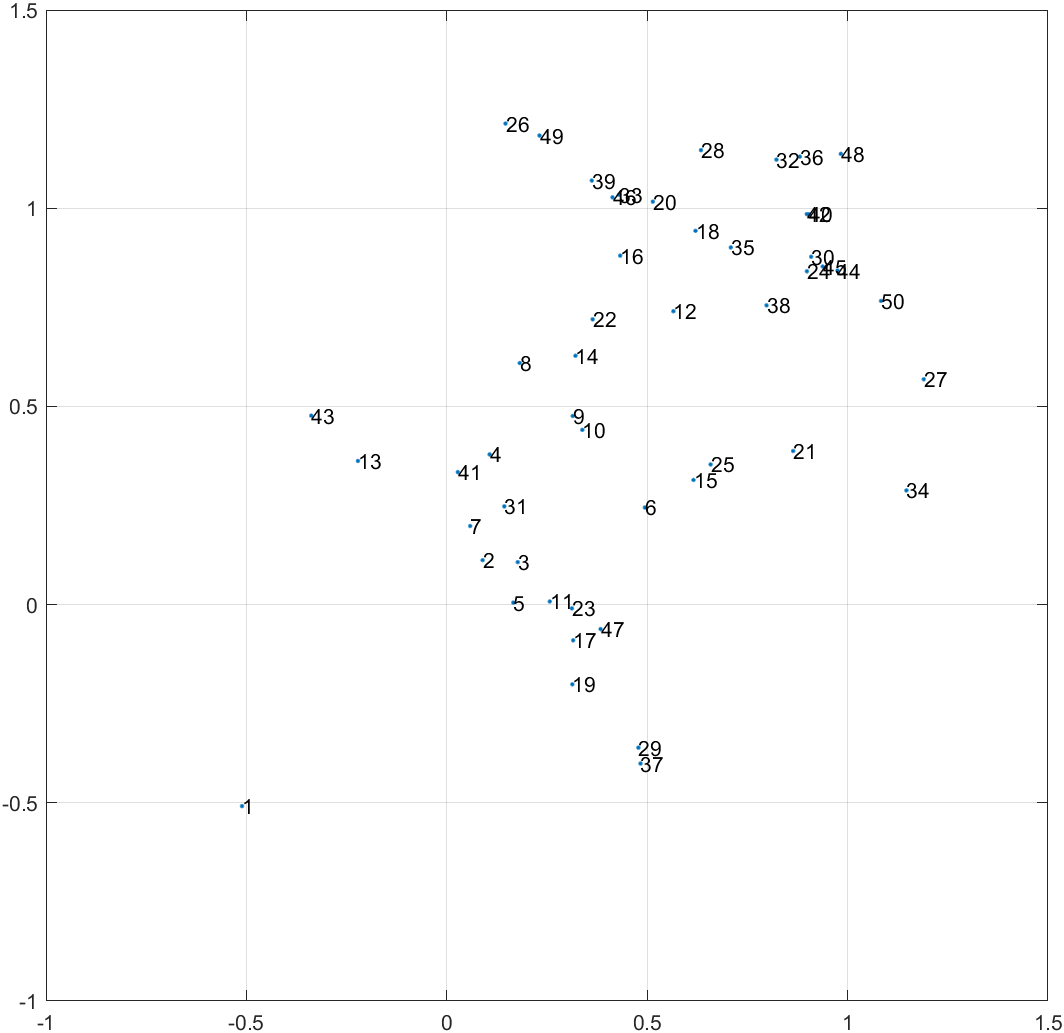
\includegraphics[width=\textwidth]{IMG/ug_50nodes.png}
        \caption{Embedding of an undirected graph with 50 nodes.}
        \label{fig:ug_50nodes}
    \end{subfigure}
    \caption{Embedding results for different types of graphs.}
    \end{center}
    % \vspace{-0mm}
\end{figure*}

Next, we simulated the embedding of a larger acyclic digraph with 50 nodes, as shown in Fig. \ref{fig:50nodes}. The embedding results are illustrated in Fig. \ref{fig:ag_50nodes}. We have a root node \(E_1\) that influences the other prime number nodes. Moreover the other numbered nodes have a role of heads that enforce their multiples. For example, \(E_2\) is enforced by \(E_1\) and \(E_2\) have out-degree relations to other even numbered nodes: \(E_4, E_6, E_8, \ldots, E_{50}\). Other nodes also have directed relations to their multiples. 

The embedding results show that all entities converged to their respective positions, confirming the stability of the embedding process for the acyclic digraph.

Finally, we simulated the embedding of an undirected version of the former graph with 50 nodes. The results are shown in Fig. \ref{fig:ug_50nodes}. All entities converged to their respective positions, confirming the stability of the embedding process for the undirected graph.








% \begin{figure*}[h] % 'h' specifies placement (here)
%     \centering
%     \begin{tikzpicture}[nodes={circle, draw, fill=white!20, scale=1.0},>=Stealth, every edge/.style={draw, ->, thick}]
%         \graph[spring layout, node sep=20mm, sibling sep=50mm] {
%             1 -> {2, 3, 5, 7, 11, 13, 17, 19, 23, 29, 31, 37, 41, 43, 47},
%             2 -> {4, 6, 8, 10, 12, 14, 16, 18, 20, 22, 24, 26, 28, 30, 32, 34, 36, 38, 40, 42, 44, 46, 48, 50},
%             3 -> {6, 9, 12, 15, 18, 21, 24, 27, 30, 33, 36, 39, 42, 45, 48},
%             4 -> {8, 12, 16, 20, 24, 28, 32, 36, 40, 44, 48},
%             5 -> {10, 15, 20, 25, 30, 35, 40, 45, 50},
%             6 -> {12, 18, 24, 30, 36, 42, 48},
%             7 -> {14, 21, 28, 35, 42, 49},
%             8 -> {16, 24, 32, 40, 48},
%             9 -> {18, 27, 36, 45},
%             10 -> {20, 30, 40, 50},
%             11 -> {22, 33, 44},
%             12 -> {24, 36, 48},
%             13 -> {26, 39},
%             14 -> {28, 42},
%             15 -> {30, 45},
%             16 -> {32, 48},
%             17 -> {34},
%             18 -> {36},
%             19 -> {38},
%             20 -> {40},
%             21 -> {42},
%             22 -> {44},
%             23 -> {46},
%             24 -> {48},
%             25 -> {50}
%         };

%     \end{tikzpicture}
%     \caption{Acyclic digraph of 50 nodes.}
%     \label{fig:50nodes}
% \end{figure*}

\section{Conclusion}
In this paper, we have proposed a novel integration of Knowledge Graph Embedding (KGE) with distributed optimization and formation control. 
By reformulating the TransE optimization problem as a distributed optimization task, we demonstrated how multi-agent systems can effectively learn embeddings while interacting only with neighboring entities. 
This approach leverages graph-theoretical concepts, specifically the properties of the graph Laplacian, to analyze the convergence and stability of the embedding process.
Our results highlight that TransE, when interpreted through the lens of distributed optimization, can be seen as a formation control problem. 
The equivalence between the gradient descent dynamics in distributed optimization and the control laws in formation control allows for a deeper understanding of the embedding process in multi-agent systems.
The use of the in-degree Laplacian matrix \(L\) provides valuable information on the stability and convergence behavior of the embedding.
Overall, this work bridges the gap between knowledge graph embedding, distributed optimization, and formation control, offering a comprehensive framework for understanding and improving the performance of KGE methods in decentralized and multi-agent environments.

In future work, we plan to explore more complex graph structures and investigate the impact of different graph properties on the stability and convergence of the embedding process. Additionally, we aim to extend our analysis to other KGE models and evaluate the effectiveness of distributed optimization in learning embeddings for various types of knowledge graphs.


\bibliographystyle{IEEEtran}
\bibliography{kge}

\end{document}